% !TEX TS-program = pdflatex
% !TEX encoding = UTF-8 Unicode

\documentclass[11pt,a4paper,english]{article} % document type and language

% Laad stijlen via relatieve paden
\newcommand{\path}{C:/Users/Admin/Documents/GitHub/Statistiek}
\usepackage{\path/LaTeX/styles/config}
\usepackage{\path/LaTeX/styles/statistics-macros}
\graphicspath{{\path/LaTeX/figures/}}

\usetikzlibrary{shapes.geometric, arrows.meta, positioning}
\setlength{\parindent}{0cm} 

\tikzstyle{startstop} = [rectangle, rounded corners, minimum width=3cm, minimum height=1cm, rounded corners, text centered, draw=black, fill=blue!20]
\tikzstyle{decision} = [rectangle, minimum width=3cm, minimum height=1cm, rounded corners, text centered, draw=black, fill=orange!30]
\tikzstyle{process} = [rectangle, minimum width=3.5cm, minimum height=1cm, rounded corners, text centered, draw=black, fill=green!20]
\tikzstyle{arrow} = [thick,->,>=stealth]

\title{Formula sheet - Probability \& Statistics (Premaster MTPS)}
\author{2026 -- 2027}
\date{}
\begin{document}
\maketitle
\section*{Probability Rules:}
\begin{center}
    \renewcommand{\arraystretch}{1.5}
    \begin{tabular}{lm{0.7\textwidth}}
        \toprule
            \textbf{Complement rule:} & $P(A') = 1 - P(A)$ \\
            \textbf{General addition rule:} & $P(A \cup B) = P(A) + P(B) - P(A \cap B)$ \\
            \textbf{Conditional probability:} & $P(A \mid B) = \frac{P(A \cap B)}{P(B)}$ \\
            \textbf{Law of total probability:} & Assume $S$ can be partitioned into $B_1$, $B_2$, $\ldots$, $B_k$: \newline
            $P(A) = \sum_{i=1}^k P(A \mid B_i) \cdot P(B_i)$ \\
            \textbf{Independence:} & for independent events $A$ and $B$: $P(A \cap B) = P(A) \cdot P(B)$\\
            \textbf{Bayes' theorem:} & $P(A \mid B) = \frac{P(B \mid A) \cdot P(A)}{P(B)}$ \\
        \bottomrule
    \end{tabular}
\end{center}

\section*{Discrete and continuous random variables:}
\begin{center}
    \renewcommand{\arraystretch}{1.8}
    \begin{tabular}{m{0.12\textwidth}m{0.43\textwidth}m{0.4\textwidth}}
        \toprule
                                                    & \textbf{Discrete random variables:}                           & \textbf{Continuous random variables:} \\ 
        \midrule
            \textbf{Sample \newline space:}         & Individual, separate values \newline e.g., $0, 1, 2, \ldots$  & Spectrum of values,\newline e.g., the interval $[0, 1]$.\\
        % \midrule
            \textbf{Application:}                   & Counting / categorizing                                       & Measurements \\
        % \midrule
            \textbf{Probability \newline concept:}  & Probability mass function $f(x) = P(X=x)$ \newline \begin{itemize} \item $f(x) \geq 0$ for all $x$ \item $\sum_{x} f(x) = 1$ \end{itemize} & Probability density function $f(x)$ \newline \begin{itemize} \item $f(x) \geq 0$ for all $x$ \item $\int_{-\infty}^{\infty} f(x) \dx = 1$ \end{itemize} \\
        % \midrule
            \textbf{CDF}                            & $F(x) = P(X \le x) = \sum\limits_{y: y \le x} f(y)$           & $F(x) = P(X \le x) = \int\limits_{y=-\infty}^{x} f(y)\dy$ \\
        % \midrule
            \textbf{Expected \newline value:}       & $E(X) = \sum\limits_{x} x \cdot f(x)$                         & $E(X) = \int\limits_{x=-\infty}^{\infty} x \cdot f(x)\dx$\\
        % \midrule
            \textbf{Variance:}                      & $V(X) = \sum\limits_{x} \left(x - E(X)\right)^2 \cdot f(x)$ \newline $V(X) = E(X^2) - \left[E(X)\right]^2$ & $V(X) = \int\limits_{x=-\infty}^{\infty} \left(x - E(X)\right)^2 \cdot f(x) \dx$ \newline $V(X) = E(X^2) - \left[E(X)\right]^2$ \\
        % \midrule
            \textbf{Standard deviation:}            & $\sigma(X) = \sqrt{V(X)}$                                     & $\sigma(X) = \sqrt{V(X)}$ \\
        \bottomrule
    \end{tabular}
\end{center}

\newpage

\section*{Common probability distributions:}

{\small
    \begin{center}
        \begin{tabular}{m{0.18\textwidth}m{0.28\textwidth}m{0.28\textwidth}m{0.05\textwidth}c}
            \toprule
                \textbf{Distribution} & \textbf{PMF/PDF} & \textbf{CDF} & \textbf{Mean} & \textbf{Variance} \\ 
            \midrule
                \multicolumn{5}{c}{\textbf{DISCRETE DISTRIBUTIONS}} \\ 
            \midrule
                Uniform($a, b$) \newline (values $x_1, \ldots, x_n$ \newline step size $d = \frac{b-a}{n-1}$) & $f(x) = \frac{1}{n}$ \newline $(x = x_1, \ldots, x_n)$ & $F(x) = \begin{cases} 
                0, & x < a, \\
                \frac{k}{n}, & x_k \leq x < x_{k+1}, \\
                1, & x \geq b.
                \end{cases}$ & $\frac{a+b}{2}$ & $d^2 \cdot \frac{n^2-1}{12}$ \\ 
            \midrule
                Bernoulli($p$) & $f(x) = \begin{cases} 1-p, & x = 0, \\ p, & x = 1. \end{cases}$ & $F(x) = \begin{cases} 
                0, & x < 0, \\
                1-p, & 0 \leq x < 1, \\
                1, & x \geq 1.
                \end{cases}$ & $p$ & $p \cdot (1-p)$ \\ 
            \midrule
                Binomial($n,p$) & $f(x) = \binom{n}{x}\cdot p^x \cdot (1-p)^{n-x}$ \newline ($x = 0, 1, \ldots, n$) & $F(x) = \sum\limits_{i=0}^x \binom{n}{i}\cdot p^i \cdot (1-p)^{n-i}$ & $n\cdot p$ & $n\cdot p\cdot (1-p)$ \\ \midrule
                Geometric($p$) & $f(x) = p \cdot (1-p)^{x-1}$ \newline ($x = 1, 2, \ldots$) & $F(x) = \sum\limits_{i=1}^x p\cdot (1-p)^{i-1}$ & $\frac{1}{p}$ & $\frac{1-p}{p^2}$ \\ \midrule
                Pois($\lambda$) & $f(x) = e^{-\lambda}\cdot \frac{\lambda^x}{x!}$ \newline ($x = 0, 1, \ldots$) & $F(x) = \sum\limits_{i=0}^x e^{-\lambda} \cdot \frac{\lambda^i}{i!}$ & $\lambda$ & $\lambda$ \\ 
            \midrule
                \multicolumn{5}{c}{\textbf{CONTINUOUS DISTRIBUTIONS}} \\ 
            \midrule
                Uniform($a, b$) & $f(x) = \begin{cases} \frac{1}{b-a}, & a \leq x \leq b, \\ 0, & \text{otherwise.} \end{cases}$ & $F(x) = \begin{cases} 
                0, & x < a, \\
                \frac{x-a}{b-a}, & a \leq x < b, \\ 1, & x \geq b. \end{cases}$ & $\frac{a+b}{2}$ & $\frac{(b-a)^2}{12}$ \\ \midrule
                $N(\mu, \sigma)$ & $f(x) = \frac{1}{\sigma\cdot\sqrt{2\pi}} e^{-\frac{1}{2}\left(\frac{x-\mu}{\sigma}\right)^2}$ & $F(x) = \Phi\left(\frac{x-\mu}{\sigma}\right)$ & $\mu$ & $\sigma^2$ \\ \midrule
                Exponential($\lambda$) & $f(x) = \begin{cases} \lambda e^{-\lambda x}, & x \geq 0, \\ 0, & \text{otherwise.} \end{cases}$ & $F(x) = \begin{cases} 1 - e^{-\lambda x}, & x \geq 0 \\ 0, & x < 0 \end{cases}$ & $\frac{1}{\lambda}$ & $\frac{1}{\lambda^2}$ \\ 
            \bottomrule
        \end{tabular}
    \end{center}
}

\section*{Joint probability distributions:}
\begin{center}
    \renewcommand{\arraystretch}{1.5}
    \begin{tabular}{lm{0.7\textwidth}}
        % \toprule
            \textbf{Marginal distributions:}    & $f_X(x) = \sum_{y} f_{X,Y}(x,y)$ (discrete) \newline $f_X(x) = \int_{y} f_{X,Y}(x,y) \dy$ (continuous) \\
            \textbf{Conditional probability:}   & $f_{X \mid Y}(x \mid y) = \frac{f_{X,Y}(x,y)}{f_Y(y)}$ (discrete) \\
            \textbf{Covariance:}                & $\Cov{X}{Y} = E\left[ (X-E(X)) \cdot (Y - E(Y))\right] = E(XY) - E(X) \cdot E(Y)$ \\
            \textbf{Correlation coefficient:}   & $\rho(X,Y) = \frac{\Cov{X}{Y}}{\sigma(X) \cdot \sigma(Y)}$ \\        
        % \bottomrule
    \end{tabular}   
\end{center}

\section*{Functions of random variables:}
\begin{center}
    \renewcommand{\arraystretch}{1.5}
    \begin{tabular}{m{0.25\textwidth}m{0.7\textwidth}}
        % \toprule
            \textbf{Linearity of \newline expectation:}  & $E(aX+bY+c) = a \cdot E(X) + b \cdot E(Y) + c $ \\
            \textbf{Variance of functions \newline of random variables:} & $V(aX+bY) = a^2 \cdot V(X) + b^2 \cdot V(Y) + 2a\cdot b\cdot  \Cov{X}{Y}$ \\
        % \bottomrule
    \end{tabular}  
\end{center}

\section*{Central limit theorem:}
Let $X_1, X_2, \ldots, X_n$ be independent and identically distributed random variables with mean $\mu$ and standard deviation $\sigma$.
Then the following holds:
\begin{itemize}
    \item the sum $\sum_{i=1}^{n} X_i = X_1 + X_2 + \ldots + X_n \approx N(n \cdot \mu, \sqrt{n} \cdot \sigma)$.
    \item the average $\overline{X} = \frac{X_1 + X_2 + \ldots + X_n}{n} \approx N(\mu, \sigma / \sqrt{n})$.
\end{itemize}

\section*{Point estimators:}
Let $\hat{\Theta}$ be an estimator (random variable) and $\hat{\theta}$ an estimate (outcome) of a population parameter $\theta$.\medskip

\begin{center}
    \renewcommand{\arraystretch}{1.8}
    \begin{tabular}{m{0.25\textwidth}m{0.7\textwidth}}
        % \toprule
            \textbf{Sample mean:} & $\overline{x} = \frac{\sum_{i=1}^{n} x_{i}}{n}$ \\
            \textbf{Sample variance:} & $s^2 = \frac{1}{n-1}\sum_{i=1}^{n} (x_{i} - \overline{x})^2$ \\
            \textbf{Bias:}  & $\textrm{Bias}(\hat{\Theta}) = E(\hat{\Theta}) - \theta$ \\
            \textbf{Standard error:} & $\textrm{SE}(\hat{\Theta}) = \sqrt{V(\hat{\Theta})}$ \\
            \textbf{Mean squared error:} & $\textrm{MSE}(\hat{\Theta}) = E\left( (\hat{\Theta} - \theta)^2\right)=  V(\hat{\Theta}) + \textrm{Bias}(\Theta)^2$ \\
            \textbf{Relative efficiency:} & $\frac{\textrm{MSE}(\hat{\Theta_1})}{\textrm{MSE}(\hat{\Theta_2})}$ \\[2ex]
            \textbf{Maximum likelihood:} & \begin{itemize}
                \item Define the likelihood function: $L(\theta) = \prod_{i=1}^n f(x_i; \theta) = f(x_1; \theta)\cdot f(x_2; \theta)\cdot\ldots\cdot f(x_n; \theta)$
                \item If necessary, take the log likelihood function $\ln{L(\theta)}$ (as products becomes sums when taking logs).
                \item Determine the value of $\theta$ that maximizes $L(\theta)$ (or $\ln{L(\theta)}$).
            \end{itemize} \\
        % \bottomrule
    \end{tabular}
\end{center}


\section*{Interval estimators:}

\begin{center}
    \begin{tabular}{m{0.4\textwidth}C{0.5\textwidth}}
    % \toprule
        \textbf{$z$-value:}  & \textbf{TI:} $z_{\alpha/2} = \invnorm(\opp=1-\alpha/2, \mu=0, \sigma=1)$ \newline \textbf{Casio:} $z_{\alpha/2} = \invnormC(\opp=1-\alpha/2, \sigma=1,\mu=0)$ \\
        \textbf{$t$-value:}  & \textbf{TI:} $t_{n-1,\alpha/2} = \invt(\opp=1-\alpha/2, \df=n-1)$ \newline \textbf{Casio:} $t_{n-1,\alpha/2} = \invtC(\opp=\alpha/2, \df=n-1)$ \\
        \textbf{$100(1-\alpha)$\si{\percent}-confidence interval (CI) for the mean $\mu$ ($\sigma$ known):} & $[\overline{X} - z_{\alpha/2} \cdot \sigma / \sqrt{n}, \quad  \overline{X} + z_{\alpha/2} \cdot \sigma / \sqrt{n}]$ \\
        \textbf{$100(1-\alpha)$\si{\percent}-confidence interval (CI) for the mean $\mu$ ($\sigma$ unknown):} & $[\overline{X} - t_{n-1,\alpha/2} \cdot S / \sqrt{n}, \quad  \overline{X} + t_{n-1,\alpha/2} \cdot S / \sqrt{n}]$ \\
        \textbf{Minimum sample size for a \newline \textbf{$100(1-\alpha)$\si{\percent}-CI with error margin $\pm E$ \newline ($\sigma$ known):}} & $n \geq \left(\frac{z_{\alpha/2}\cdot \sigma}{E}\right)^2$ \\
        \textbf{Minimum sample size for a \newline \textbf{$100(1-\alpha)$\si{\percent}-CI with error margin $\pm E$ \newline ($\sigma$ unknown):}} &
        \begin{itemize} 
            \item Determine initial value for $n$ using formula above (as if $\sigma = s$).
            \item Fill in $y_1 = s / \sqrt{X} \cdot t_{X-1, \alpha/2}$ (see $t$-value). 
            \item Generate table starting from initial value and determine the smallest $n$ such that $y_1 \leq E$. 
        \end{itemize} \\
    \end{tabular}  
\end{center}

\newpage

\section*{Hypothesis testing}
\begin{center}
    \renewcommand{\arraystretch}{1.5}
    \begin{tabular}{m{0.2\textwidth}m{0.25\textwidth}m{0.40\textwidth}}
        \toprule
            \textbf{Test name} & \textbf{Test statistic} & \textbf{Probability distribution (under $H_0$)} \\
        \midrule
            \multicolumn{3}{c}{\textbf{Tests for the mean $\mu$ of a normal distribution}} \\ 
        \midrule
            $\sigma$ known    & $Z = \frac{\overline{X} - \mu_0}{\sigma / \sqrt{n}}$ & $N(0, 1)$ \\
            $\sigma$ unknown  & $T = \frac{\overline{X} - \mu_0}{S / \sqrt{n}}$ & $t(\df=n-1)$ \\
        \midrule
            \multicolumn{3}{c}{\textbf{Chi-square test ($\chi^2$)}} \\
        \midrule
            Chi-square \newline goodness-of-fit & $X^2 = \sum_{i} \frac{(O_{i} - E_{i})^2}{E_{i}}$ & $\chi^2\left(\df=\text{\#categories-1}\right)$ \\
        \midrule
            \multicolumn{3}{c}{\textbf{Correlation test ($\rho = 0$)}} \\ 
        \midrule
            Significant \newline correlation & $T = \frac{R \sqrt{n-2}}{\sqrt{1-R^2}}$ & $t(\df=n-2)$ \\
        % \midrule
            % \midrule
        %     \multicolumn{4}{c}{\textbf{Toetsen op basis van twee onafhankelijke populaties $A$ en $B$ (met steekproefgroottes $n$ en $m$)}} \\
        % \midrule
        %     $F$-toets & $\sigma_A^2 = \sigma_B^2$ & $F = \frac{S_A^2}{S_B^2}$ & $F\left(\df_A = n-1, \df_B = m-1\right)$ \\
        %     $z$-toets & $\mu_A \leq/=/\geq \mu_B$ & $Z = \frac{(\overline{X_A} - \overline{X_B}) - (\mu_A - \mu_B)}{\sqrt{\frac{\sigma_A^2}{n} + \frac{\sigma_B^2}{m}}}$ & $N\left(\mu=0, \sigma=1\right)$ \\
        %     $t$-toets ($\sigma_A^2 = \sigma_B^2$) & $\mu_A \leq/=/\geq \mu_B$ & $T = \frac{(\overline{X_A} - \overline{X_B}) - (\mu_A - \mu_B)}{\sqrt{\frac{S_P^2}{n} + \frac{S_P^2}{m}}}$ & $t\left(\df=n+m-2\right)$ \\
        %     $t$-toets ($\sigma_A^2 \neq \sigma_B^2$) & $\mu_A \leq/=/\geq \mu_B$ & $T = \frac{(\overline{X_A} - \overline{X_B}) - (\mu_A - \mu_B)}{\sqrt{\frac{S_A^2}{n} + \frac{S_B^2}{m}}}$ & $t\left(\df=\min(n-1, m-1)\right)$ \\
        \bottomrule
    \end{tabular}
\end{center}

\textbf{One-sided and two-sided hypothesis tests}
\begin{center}
    \begin{tabular}{@{}c@{}c@{}c@{}}
        \textbf{Left-sided} & \textbf{Two-sided} & \textbf{Right-sided} \\
        $H_0: \mu \geq \mu_0 \text{ vs. } H_1: \mu < \mu_0$ & $H_0: \mu = \mu_0 \text{ vs. } H_1: \mu \neq \mu_0$ & $H_0: \mu \leq \mu_0 \text{ vs. } H_1: \mu > \mu_0$ \\
        Acceptance region: {\color{green!50!black} $[g, \infty)$} & Acceptance region: {\color{green!50!black} $[g_1, g_2]$} & Acceptance region: {\color{green!50!black} $(-\infty, g]$} \\
        Critical region: {\color{red} $(-\infty, g)$} & Critical region: {\color{red} $(-\infty, g_1)$ and $(g_2, \infty)$} & Critical region: {\color{red} $(g, \infty)$} \\
        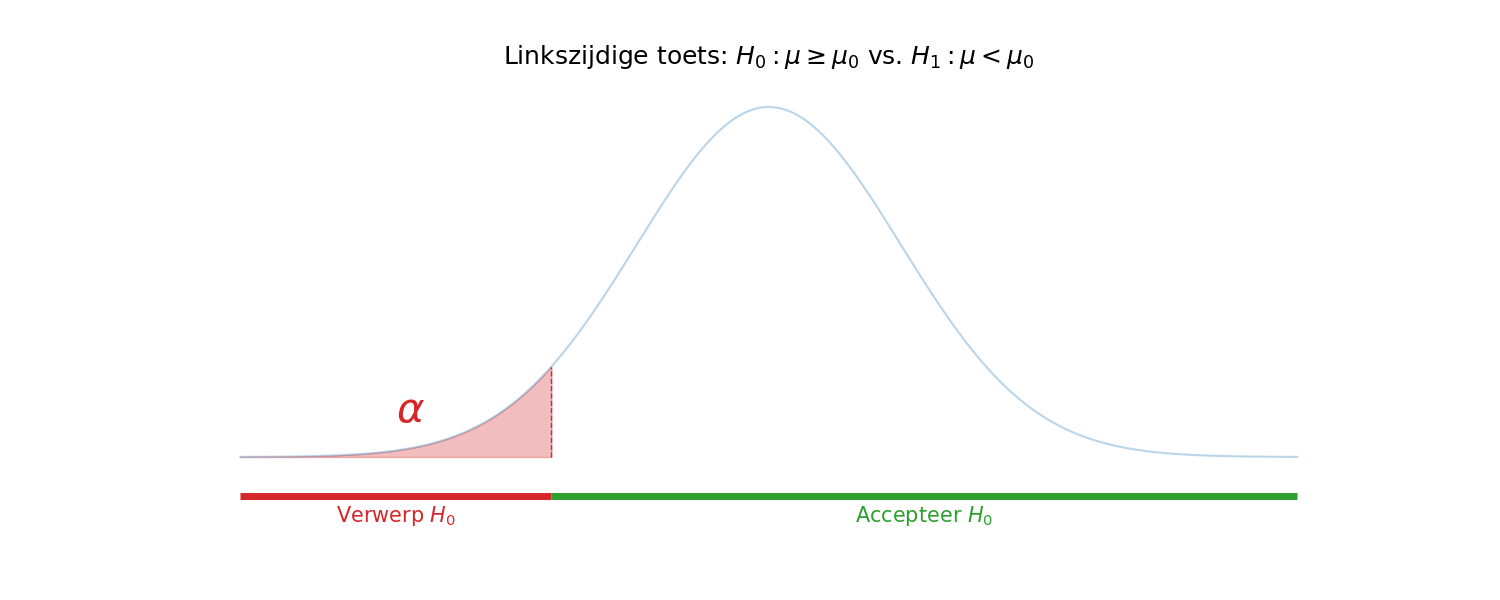
\includegraphics[width=0.33\textwidth]{../../LaTeX/figures/linkszijdig.png} & 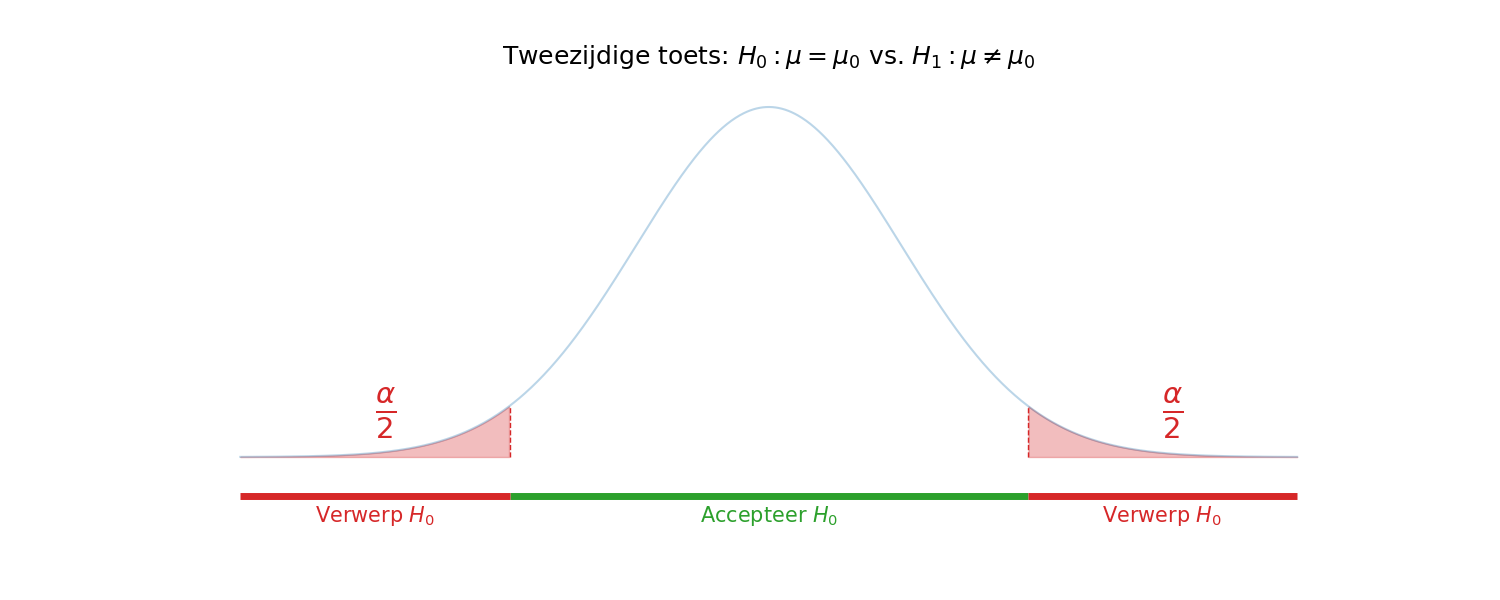
\includegraphics[width=0.33\textwidth]{../../LaTeX/figures/tweezijdig.png} & 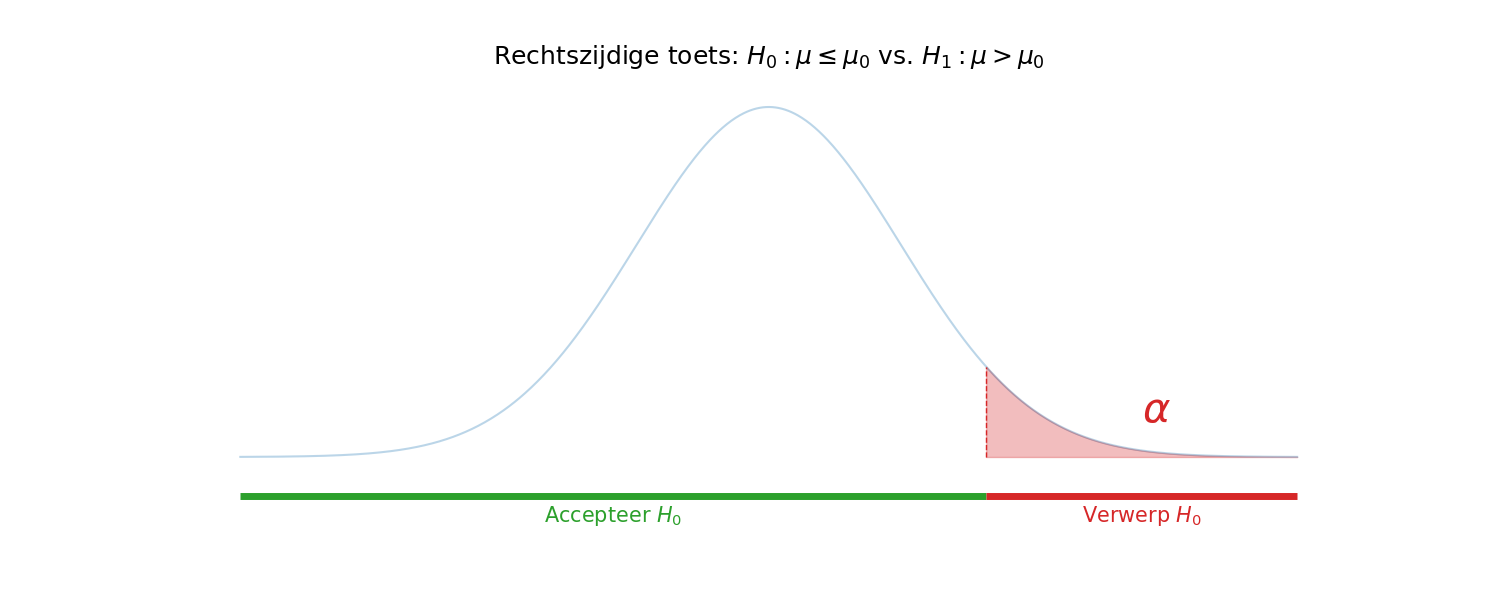
\includegraphics[width=0.33\textwidth]{../../LaTeX/figures/rechtszijdig.png}\\
    \end{tabular}
\end{center}

\textbf{Critical regions:}
    \begin{center}
        \renewcommand{\arraystretch}{1.5}
        \begin{tabular}{m{.13\textwidth}|m{.14\textwidth}|m{.23\textwidth}|m{.35\textwidth}}
            \toprule
                \textbf{Probability distribution (under $H_0$)} & \textbf{Left-sided} \newline $(-\infty, g)$ & \textbf{Two-sided} \newline $(-\infty, g_1)$ and $(g_2, \infty)$ & \textbf{Right-sided} \newline $(g, \infty)$ \\
            \midrule
                $N\left(0, 1\right)$ & $\invnorm$ with \newline $\opp=\alpha$ & $\invnorm$ with \newline $\opp=\alpha/2$ and $1-\alpha/2$ & $\invnorm$ with \newline $\opp=1-\alpha$ \\
            \midrule
                $t(\df)$ & $\invt$ with \newline $\opp=\alpha$ & $\invt$ with \newline $\opp=\alpha/2$ and $1-\alpha/2$ & $\invt$ with \newline $\opp=1-\alpha$ \\
            \midrule
                \multicolumn{4}{c}{\emph{Critical region that needs to be solved with the \enquote{numeric solver} or \enquote{SolveN}:}} \\
            \midrule
                $\chi^2(\df)$ & - & - & \textbf{TI:} $\chi^2\text{cdf}(g, 10^{99}, \df) = \alpha$ or \textbf{Casio:} \newline $\textrm{SolveN}(\textrm{ChiCD}(x, 10^{99}, \df)=\alpha,x)$ \\
            \bottomrule
        \end{tabular}
    \end{center}

    \emph{N.B.: when using Casio: (i) the order is $\sigma$, $\mu$, and (ii) $\invtC$ computes boundary values with area on the right, so replace $\opp$ by $1 - \opp$ where applicable.}

\newpage

\textbf{$p$-values}
\begin{center}
    \renewcommand{\arraystretch}{1.5}
    \begin{tabular}{m{.13\textwidth}m{.09\textwidth}m{.16\textwidth}m{.29\textwidth}m{.16\textwidth}}
        \toprule
            \textbf{Probability distribution (under $H_0$)} & \textbf{Test \newline statistic} & \textbf{Left-sided} & \textbf{Two-sided} & \textbf{Right-sided} \\
        \midrule
            $N(0, 1)$ & $Z$ & $p = P(Z \leq z)$ & $p =$ minimum of \newline  $P(Z \leq z)$ and $P(Z \leq z)$ & $p = P(Z \geq z)$ \\
        \midrule
            $t(\df)$ & $T$ & $p = P(T \leq t)$ & $p =$ minimum of \newline $P(T \leq t)$ and $P(T \leq t)$ & $p = P(T \geq t)$\\
        \midrule
            $\chi^2(\df)$ & $X^2$ & $p = P(X^2 \leq \chi^2)$ & $p =$ minimum of \newline $P(X^2 \leq \chi^2)$ and $P(X^2 \leq \chi^2)$ & $p = P(X^2 \geq \chi^2)$\\
            & & Compare with $\alpha$ & Compare with $\alpha/2$ & Compare with $\alpha$ \\
        \bottomrule
    \end{tabular}
\end{center}

\section*{Type-II errors}
\begin{center}
    \begin{tabular}{m{0.3\textwidth}m{0.65\textwidth}}
        \textbf{Type-II error $\beta$ for a $z$-test (given $H_1: \mu = \mu_1$):} & \begin{itemize}\setlength\itemsep{1em}
        \item Transform critical region for $N(0,1)$ to a critical region for $N(\mu_0, \sigma / \sqrt{n})$ using $x \mapsto \mu_0 + x \cdot \sigma / \sqrt{n}$.
        \item $\beta = 1 - P(\overline{X} \text{ in critical region } | \mu = \mu_1)$ \newline $= 1 - \normalcdf(\ldots, \ldots, \mu_1, \sigma / \sqrt{n})$
    \end{itemize}\\
        \textbf{Minimum sample size $n$ such that $\beta \leq \beta_0$ and $\mu_1 = \mu_0 + \delta$:} & $n \geq \left( \frac{(z_{\alpha/2} + z_{\beta_0}) \cdot \sigma}{\delta}\right)^2$
    \end{tabular} 
\end{center}

\section*{Linear regression and correlation}
\begin{center}
    \renewcommand{\arraystretch}{1.8}
    \begin{tabular}{m{0.3\textwidth}m{0.6\textwidth}}
        % \toprule
        \textbf{Simple linear regression \newline model:} & $Y = \beta_0 + \beta_1 \cdot x + \epsilon$ \\
        \textbf{Least squares coefficients:} & $\hat{\beta}_{1} = \frac{\sum_{i=1}^{n}x_iy_i - n \cdot \overline{x} \cdot \overline{y}}{\sum_{i=1}^{n} x_{i}^2 - n \cdot \overline{x}^2} = \frac{\overline{xy}-\overline{x}\cdot \overline{y}}{\overline{x^2}-\overline{x}^2}$ \newline
                                                $\hat{\beta}_{0} = \overline{y} - \hat{\beta}_{1} \cdot \overline{x}$ \\
        \textbf{Variance of error terms:} & $\hat{\sigma}^2 = \frac{1}{n-2}\sum_{i=1}^{n} (y_{i} - \hat{y}_{i})^2 = \frac{\sum_{i=1}^{n} y_{i}^2 - \hat{\beta}_{0}\cdot \sum_{i=1}^{n} y_{i} - \hat{\beta}_{1}\cdot \sum_{i=1}^{n} x_{i}y_{i}}{n-2}$ \\
        \textbf{Pearson's correlation \newline coefficient:} & $r(x, y) = \frac{\Cov{x}{y}}{\sqrt{s_{X}^2\cdot s_{Y}^2}} = \frac{\overline{xy} - \overline{x} \cdot \overline{y}}{\sqrt{(\overline{x^2} - \overline{x}^2)\cdot(\overline{y^2} - \overline{y}^2)}}$
        % \bottomrule
    \end{tabular}
\end{center}

\end{document}
